\documentclass[a4paper,12pt]{article}
\usepackage{graphicx}
\usepackage{epstopdf}
\usepackage{longtable}
\usepackage{float}
\usepackage{breakurl}
\usepackage{tabularx}
\usepackage[colorlinks=false]{hyperref}
%% Definitioner för LIPS-dokument

\usepackage[swedish]{babel}
\usepackage[utf8]{inputenc}
\usepackage[T1]{fontenc}
\usepackage{times}
\usepackage{ifthen}

\usepackage[margin=25mm]{geometry}

\usepackage{fancyhdr}
\pagestyle{fancy}
\lhead{}
\chead{\textbf{\LIPSprojekttitel}}
\rhead{\textbf{\textsl{LiTH}}\\\textbf{\LIPSdatum}}
\lfoot{\textbf{\LIPSkursnamn}\\\textbf{\LIPSdokumentansvarig}}
\cfoot{\textbf{\LIPSprojektgrupp}\\\textbf{\LIPSgruppepost}}
\rfoot{\textbf{\textsc{Lip}s}\\\textbf{Sida~\thepage}}

\setlength{\parindent}{0pt}
\setlength{\parskip}{1ex plus 0.5ex minus 0.2ex}


\newcommand{\twodigit}[1]{\ifthenelse{#1<10}{0}{}{#1}}
\newcommand{\dagensdatum}{\number\year-\twodigit{\number\month}-\twodigit{\number\day}}

%% ------------------------------------------
% NYBILD
% Skapar centrerad bild med caption
%   
% #1: Filens url relativt '/bilder/'
% #2:  Caption
% #3: Label
% #4: Skalning
%% ------------------------------------------
\newcommand{\nyBild}[4] 
{\begin{figure}[H]
  \centering
 \includegraphics[angle=0,scale=#4]{bilder/#1}
  \caption{#2}
  \label{fig:#3}
\end{figure}}



%%  Redefinitions of commands containing @
\makeatletter
\makeatother

\newcommand{\LIPStitelsida}{%
{\ }\vspace{45mm}
\begin{center}
  \textbf{\Huge \LIPSdokumenttyp}
\end{center}
\begin{center}
  {\Large Redaktör: \LIPSredaktor}
\end{center}
\begin{center}
  {\Large \textbf{Version \LIPSversion}}
\end{center}
\vfill
\begin{center}
  {\large Status}\\[1.5ex]
  \begin{tabular}{|*{3}{p{40mm}|}}
    \hline
    Granskad & \LIPSgranskare & \LIPSgranskatdatum \\
    \hline
    Godkänd & \LIPSgodkannare & \LIPSgodkantdatum \\
    \hline
  \end{tabular}
\end{center}
\newpage
}


\newenvironment{LIPSprojektidentitet}{%
{\ }\vspace{45mm}
\begin{center}
  {\Large PROJEKTIDENTITET}\\[0.5ex]
  {\small
  \LIPSartaltermin, \LIPSprojektgrupp\\
  Linköpings Tekniska Högskola, ISY
  }
\end{center}
\begin{center}
  {\small Gruppdeltagare}\\
%  \begin{tabular}{|p{30mm}|p{40mm}|p{35mm}|p{45mm}|}
  \begin{tabular}{|l|p{45mm}|p{25mm}|l|}
    \hline
    \textbf{Namn} & \textbf{Ansvar} & \textbf{Telefon} & \textbf{E-post} \\
    \hline
}%
{%
    \hline
  \end{tabular}
\end{center}
\begin{center}
  {\small
    \textbf{E-postlista för hela gruppen}: \LIPSgruppepost\\
    \textbf{Hemsida}: \LIPSgrupphemsida\\[1ex]
    \textbf{Kund}: \LIPSkund\\
    \textbf{Kontaktperson hos kund}: \LIPSkundkontakt\\
    \textbf{Kursansvarig}: \LIPSkursansvarig\\
    \textbf{Handledare}: \LIPShandledare\\
  }
\end{center}
\newpage
}
\newcommand{\LIPSgruppmedlem}[4]{\hline {#1} & {#2} & {#3} & {#4} \\}



\newenvironment{LIPSdokumenthistorik}{%
\begin{center}
  Dokumenthistorik\\[1ex]
  \begin{small}
    \begin{tabular}{|l|l|p{60mm}|l|l|}
      \hline
      \textbf{Version} & \textbf{Datum} & \textbf{Utförda förändringar} & \textbf{Utförda av} & \textbf{Granskad} \\
      }%
    {%
      \hline
    \end{tabular}
  \end{small}
\end{center}
}
\newcommand{\LIPSversionsinfo}[5]{\hline {#1} & {#2} & {#3} & {#4} & {#5} \\}

\newcounter{LIPSkravnummer}
\newcounter{LIPSunderkravnummer}[LIPSkravnummer]
\newenvironment{LIPSkravlista}{%
  \begin{tabular}{|p{25mm}|p{25mm}|p{85mm}|p{5mm}|}
    }%
  {%
    \hline
  \end{tabular}
}
\newcommand{\LIPSkrav}[3]{\hline\stepcounter{LIPSkravnummer}\textbf{Krav nr \arabic{LIPSkravnummer}} & \textbf{{#1}} & {#2} & \textbf{{#3}} \\}
\newcommand{\LIPSunderkrav}[3]{\hline\stepcounter{LIPSunderkravnummer}\textbf{Krav nr \arabic{LIPSkravnummer}\Alph{LIPSunderkravnummer}} & \textbf{{#1}} & {#2} & \textbf{{#3}} \\}





%%% Local Variables: 
%%% mode: latex
%%% TeX-master: "kravspec_mall"
%%% End: 


\newcommand{\LIPSartaltermin}{2011/HT}
\newcommand{\LIPSkursnamn}{TSEA29}

\newcommand{\LIPSprojekttitel}{Kartrobot}

\newcommand{\LIPSprojektgrupp}{Grupp 11}
\newcommand{\LIPSgruppepost}{cajla322@student.liu.se}
\newcommand{\LIPSgrupphemsida}{finns ej}
\newcommand{\LIPSdokumentansvarig}{Sebastian Thorarensen}

\newcommand{\LIPSkund}{ISY, Linköpings universitet, 581\,83 Linköping}
\newcommand{\LIPSkundkontakt}{Ola Dahl, 013-282692, ola.dahl@liu.se}
\newcommand{\LIPSkursansvarig}{Tomas Svensson, 013-281368, tomass@isy.liu.se}
\newcommand{\LIPShandledare}{Anders Nilsson, 013-282635, andersn@isy.liu.se}

\newcommand{\LIPSdokumenttyp}{Designspecifikation}
\newcommand{\LIPSredaktor}{Sebastian Thorarensen}
\newcommand{\LIPSversion}{1.1}
%\newcommand{\LIPSdatum}{2004-xx-yy}
\newcommand{\LIPSdatum}{\dagensdatum}

% Förslag till versionshantering:
% döp helt enkelt om filen till [dokument]_vX.Y.tex vid varje revision

\newcommand{\LIPSgranskare}{}
\newcommand{\LIPSgranskatdatum}{}
\newcommand{\LIPSgodkannare}{}
\newcommand{\LIPSgodkantdatum}{}

\begin{document}

\LIPStitelsida

%% Argument till \LIPSgruppmedlem: namn, roll i gruppen, telefonnummer, epost
\begin{LIPSprojektidentitet}
  \LIPSgruppmedlem{Caj Larsson}{Projektledare (PL)}{072-2022102}
  		{cajla304@student.liu.se}
  \LIPSgruppmedlem{Sebastian Thorarensen}{Dokumentansvarig (DOK),
  		AVR-mjukvaruansvarig}{0733-567850}{sebth181@student.liu.se}
  \LIPSgruppmedlem{David Stenberg}{Beagleboard-mjukvaruansvarig}
  		{070-5369714}{davst636@student.liu.se}
  \LIPSgruppmedlem{Hannes Boberg}{Hårdvaruansvarig}
  		{0734-349419}{hanbo552@student.liu.se}
  \LIPSgruppmedlem{Erik Lindholm}{Testansvarig (TEST)}{0768-078785}
  		{erili322@student.liu.se}
  \LIPSgruppmedlem{Andreas Ölund}{AI-arktitekt}
  		{0766-292816}{andol860@student.liu.se}
  \LIPSgruppmedlem{Carl Ehrenstråhle}{Leveransansvarig, 
  		PC-mjukvaruansvarig}{070-3355560}{careh585@student.liu.se}
\end{LIPSprojektidentitet}

\tableofcontents{}
\newpage

%% Argument till \LIPSversionsinfo: versionsnummer, datum, ändringar, utfört av, granskat av
\addcontentsline{toc}{section}{Dokumenthistorik}
\begin{LIPSdokumenthistorik}
  \LIPSversionsinfo{0.1}{2011-10-26}{Första utkast.}{sebth181}{davst636}
  \LIPSversionsinfo{1.0}{2011-10-26}{Första version.}{sebth181}{davst636}
  \LIPSversionsinfo{1.1}{2011-11-14}{Andra version; ändrat dataformat för
  		kartdata}{sebth181}{davst636}
\end{LIPSdokumenthistorik}
\newpage

\section{Inledning}
Text här

\section{Systemet i sin helhet}

Roboten är baserad på det fyrhjuliga chassit ``Terminator''. Dess inbyggda
strömkälla är stor nog att kunna driva hela roboten. Elektroniken är monterad
på virkort som sitter fast på robotens ovansida.

Sensorer som används är optiska avståndsmätare, optiska hjulsensorer och gyron.

\subsection{Bussar}

Kart- och kommunikationsmodulen -- refererad till som kartmodulen -- är baserad
på en Beagleboard xM och är navet i all kommunikation moduler emellan. Alla
moduler är inkopplade till beagleboarden enligt följande tabell:

\begin{table}[h!]
	\begin{tabular}{l l}
		\textbf{Port} & \textbf{Beskrivning} \\
		Serieport     & Anslutning till sensormodul \\
		USB$\rightarrow$Serie    & Anslutning till styrmodul \\
		USB           & Blåtandssticka \\
		USB           & USB-mus \\
	\end{tabular}
\end{table}

% !TEX encoding = UTF-8 Unicode

%% --------------------------------------------------------------------------------------------------------------------------------------------
% Protokoll - En beskrivning av de protokoll som används för kommunikationen, och vad de är bra för.
%
%
% --marlo265, 2012-05-06
%% --------------------------------------------------------------------------------------------------------------------------------------------
 
\section{Protokoll}
\label{sec:protokoll}

För att förenkla kommunikation mellan enheter så används ett enhetligt
protokoll, detta gör det också väldigt mycket lättare att lägga till fler
enheter till roboten.


\subsection{Generell överföring mellan enheter}
Kommunikationen mellan de olika enheterna sker via en SPI-buss (se 
\ref{sec:SPI}).
All kommunikation består av en headerbyte följt av en databyte.
I headerbyten anges till vilken enhet den efterföljande informationen ska, 
samt hur den ska tolkas av den mottagande enheten.
De tre mest signifikanta bitarna i headern anger till vilken enhet 
informationen ska och de 5 minst signifikanta bitarna anger 
hur denna information ska behandlas. Uppdelningen kan ses i tabell 
\ref{tab:header}.  Kodningen av de tre mest signifikanta bitarna kan ses i 
tabell \ref{tab:headerkod}.

All kommunikation går via kommunikationsenheten, så om sensorenheten vill 
skicka data till styrenheten skickar den en headerbyte med styrenhetens adress 
och en databyte till kommunikationsenheten som 
tolkar headern och skickar headern och databyten till styrenheten.
\begin{table}[h]
  \centering
  \begin{tabular}{| c | c | c | c | c | c |}
    \hline
    Målenhet [3 bitar] & A & B & C & D & E \\
    \hline
  \end{tabular}
  \caption{Bituppdelning av header}
  \label{tab:header}
\end{table}

\begin{table}[h]
  \centering
  \begin{tabular}{l l}
    \textbf{3 MSB} & \textbf{Målenhet} \\
    000 & Kommunikationsenhet \\
    001 & Sensorenhet \\
    010 & Styrenhet \\
    100 & PC \\
    110 & PC och Styrenhet\\
  \end{tabular}
  \caption{Kodning av header}
  \label{tab:headerkod}
\end{table}


\subsection{PC-mjukvara $\longleftrightarrow$ Styrenhet}
Då styr- eller sensorenheten sänder data till PC-mjukvaran kommer mjukvaran att
översätta header-byten samt data-byten så att man enkelt kan åskådliggöra
instruktionen som sändes. 
PC-mjukvaran skickar styrkommandon till roboten då roboten är i fjärrstyrt läge.
Bituppdelningen av styrkommandon kan ses i tabell \ref{tab:styrbitar} och
kodningen kan ses i tabell \ref{tab:styrkommando}.

Om styrenheten får en header den inte känner igen så skickar den ett
felmeddelande till PCn.

\begin{table}[h] 
  \centering
  \begin{tabular}{| c | c |}
    \hline
    Kommando [4 bitar] & Hastighet [4 bitar] \\ \hline
  \end{tabular}
  \caption{Bituppdelning av styrkommandon}
  \label{tab:styrbitar}
\end{table}

\begin{table}[h] 
  \centering
  \begin{tabular}{l l}
    \textbf{4 MSB} & \textbf{Kommando} \\
    0000 & Stopp \\
    0001 & Framåt \\
    0010 & Fram vänster \\
    0011 & Fram höger \\
    0100 & Rotera vänster \\
    0101 & Rotera höger \\
    0110 & Back \\
    0111 & Set_left \\
    1000 & Set_right \\
    1001 & Trim_left \\
    1010 & Trim_right \\
    1011 & No_trim \\
  \end{tabular}
  \caption{Kommandokodning}
  \label{tab:styrkommando}
\end{table}


\subsection{PC-mjukvara $\longleftrightarrow$ Sensorenhet}
När sensorenheten skickar information till styrenheten och PCn 
så anger E-flaggan om roboten är i autonomt eller fjärrstyrt läge.
D-flaggan avgör om databyten som mottagits är ett specialkommando eller inte.
A-flaggan anger om roboten kör i labyrint eller om den följer en linje.
Flaggornas lägen kan ses i tabell \ref{tab:adeflaggor}.


PC-mjukvaran skickar data till sensorenheten då tröskelvärdet på linjesensorerna
kalibreras, se \ref{sec:linjesensor}.

\begin{table}[h]
  \centering
  \begin{tabular}{l l l l l l l l}
    \textbf{A} & \textbf{Läge} & & \textbf{D} & \textbf{Typ av data} & & \textbf{E} & \textbf{Läge} \\
    0 & Labyrint & & 0 & Sensordata & & 0 & Fjärrstyrt \\
    1 & Linje & & 1 & Specialkommando & & 1 & Autonomt \\
  \end{tabular}
  \caption{A-,D- och E-flaggor}
  \label{tab:adeflaggor}
\end{table}


\subsection{Sensorenhet $\longleftrightarrow$ Kommunikationsenhet}
Sensorenheten skickar data till kommunikationsenheten som ska vidare både 
till PCn och styrenheten. Detta anges med en header enligt tabell 
\ref{tab:headerkod}. Efterföljande data är antingen ett specialkommando, se 
tabell \ref{tab:special}, avstånd till väggar eller avstånd till centrumlinjen.

\begin{table}[h] 
  \centering
  \begin{tabular}{| c | c | c | c | c | c |}
    \hline
     0 & Specialkommando [3 bitar] & 0 & 0 & 0 & 0 \\ \hline
  \end{tabular}
  \caption{Bituppdelning av specialkommandon}
  \label{tab:specialbitar}
\end{table}

\begin{table}[h]
  \centering
  \begin{tabular}{l l}
    \textbf{Kodning} & \textbf{Specialkommando} \\
    000 & Återuppta vanlig reglering\\
    001 & Kör rakt fram \\
    010 & Sväng höger 90\degree \\
    011 & Sväng vänster 90\degree \\
    100 & Rotera höger 90\degree \\
    110 & Rotera vänster 90\degree \\
  \end{tabular}
  \caption{Kodning av specialkommandon}
  \label{tab:special}
\end{table}


\section{Kommunikations- och kartnavigeringsmodul}

Kartmodulen består av en Beagleboard xM och hanterar kartlogik, styr sensor-
och styrmodulen; samt kommunicerar med PC-mjukvaran.

\subsection{Hårdvara}
%Känns lite hurp durp, men det ska ju vara specat
Beagleboardens DC-anslutning kräver 5 V, 350 mA och är ansluten till
robotchassits inbyggda spänningsregulator.

För att implementera de två kontrollknapparna på roboten används knapparna på
en USB-mus användas. Mjukvaran fångar upp mushändelser. 

\subsection{Mjukvara}

\subsubsection{Operativsystem}

Vi ska använda standarddistributionen Ångström på Beagleboarden.

\subsubsection{Övrig mjukvara}

Under utvecklingsfasen används hjälpverktyg så som OpenSSH,
versionshanteringssystem, kompilatorer och textredigerare.

För att hantera USB- till serieomvandlaren och blåtandsstickan behövs
eventuellt drivrutiner.

Blåtandskommunikation hanteras med blåtandsstacken BlueZ. BlueZ möjliggör
för i princip vanlig sockelprogrammering för blåtandskommunikation i C.
% TODO ref http://people.csail.mit.edu/albert/bluez-intro/c404.html

För att hantera mushändelser används GPM.

\subsubsection{Egentuvecklad mjukvara}
Mjukvaran i kartmodulen är nästan uteslutande skriven i C. Mindre saker så som
start av robot och hantering av robotens program skrivs i shellskript.

Eftersom att kartmodulen styr roboten, hanterar reglerloop och kontinuerligt
kommunicerar med PC-mjukvaran, blir det svårt att implementera allt detta i ett
program. Mjukvaran är därför att uppdelad i olika program, vilket möjliggör
större utvecklingsparallellisering. Eftersom att roboten arbetar i två olika
lägen, fjärrstyrningsläget och det autonoma läget, så utvecklas dessa separat.

Lägesvalet hanteras av ett masterprogram. Masterprogrammet agerar även
mellanlager för I/O-hantering på roboten.

Högst prioritet i det autonoma läget har hanteringen av styr- och
sensormodulen. Blåtandshantering, d.v.s. att skicka över kartinformation till
datorn, är inte lika tidskritiskt. Mjukvaran för det autonoma läget är uppdelad
i två delar: dels ett huvudprogram som hanterar kartlogik, och dels ett program
för att hantera blåtandskommunikation med PC-mjukvaran. Kartlogikprogrammet
uppdaterar kontinuerligt en fill innehållandes kartdata som blåtandsprogrammet
läser av när PC-mjukvaran begär kartan.

Reglerloopen måste kontinuerligt efterfråga sensordata från sensormodulen. För
att reglerloopen ska fungera bäst så ska den ha ny sensordata för varje
uppdatering.

%\subsection{Blåtandshantering}
% Typ köra RFCOMM för att det är enkelt

\subsection{Kartalgoritmer}

Roboten måste dels kunna rita ut en kartan och hålla koll på sin
nuvarande position. Eftersom att kartan roboten ska ritas ut är har vissa
kraftigt begränsade egenskaper, så som väggdimensioner och endast 90-graders
vinklar, så kan implementationen av kartalgoritmen förenklas.

Kartalgoritmen ska skapa en förenklad matris som representerar 80x80 cm stora
block. För denna antas startpositionen vara i origo.

% Kolla FastSLAM, kanske lite överdriven för just vårt problem.
% http://tinyurl.com/5wesprc

% !TEX encoding = UTF-8 Unicode

\section{Sensorenhet}

Sensorenheten är den enhet som behandlar all sensordata. Den samlar in data från 
avståndssensorerna och linjesensorerna som den sedan antingen omvandlar till 
cm värden i avståndsensorns fall, eller trösklar och ger diskreta varierande storheter 
som i linjesensorns fall. Linje sensorn kommunicerar sedan med kommunikationsenheten
som förmedlar värdena till styrenheten och till PCn.

\subsection{Hårdvara}

\begin{figure}[H]
  \centering
 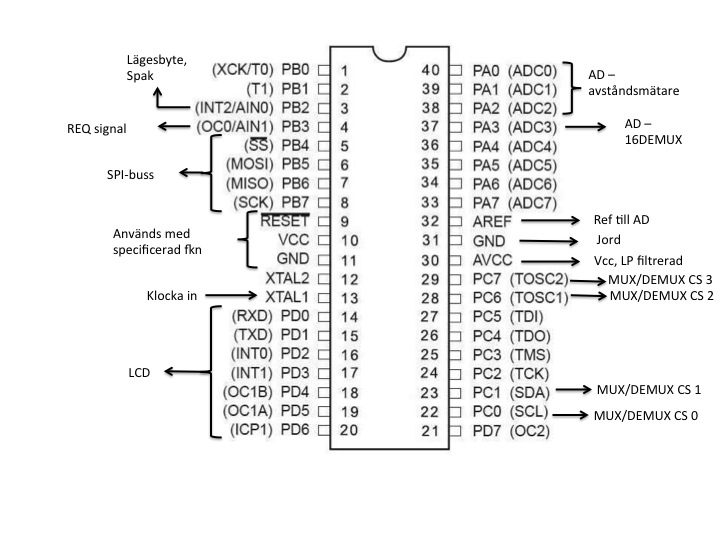
\includegraphics[angle=0,scale=0.5]{bilder/PIN_sensor.jpg}
  \caption{Sensorsenhetens pin-anslutningar}
  \label{fig:PINsensor}
\end{figure}

\subsubsection{Linjeföljarsensor}
För att maximera robotens framförhållning är sensorerna monterade framför roboten 
så långt fram som möjligt ca 3 mm ovanför marken. Linjesensorn består av 11st lysdioder 
med 11st ljuskänsliga transistorer, en multiplex och en demultiplex.

\begin{figure}[H]
  \centering
 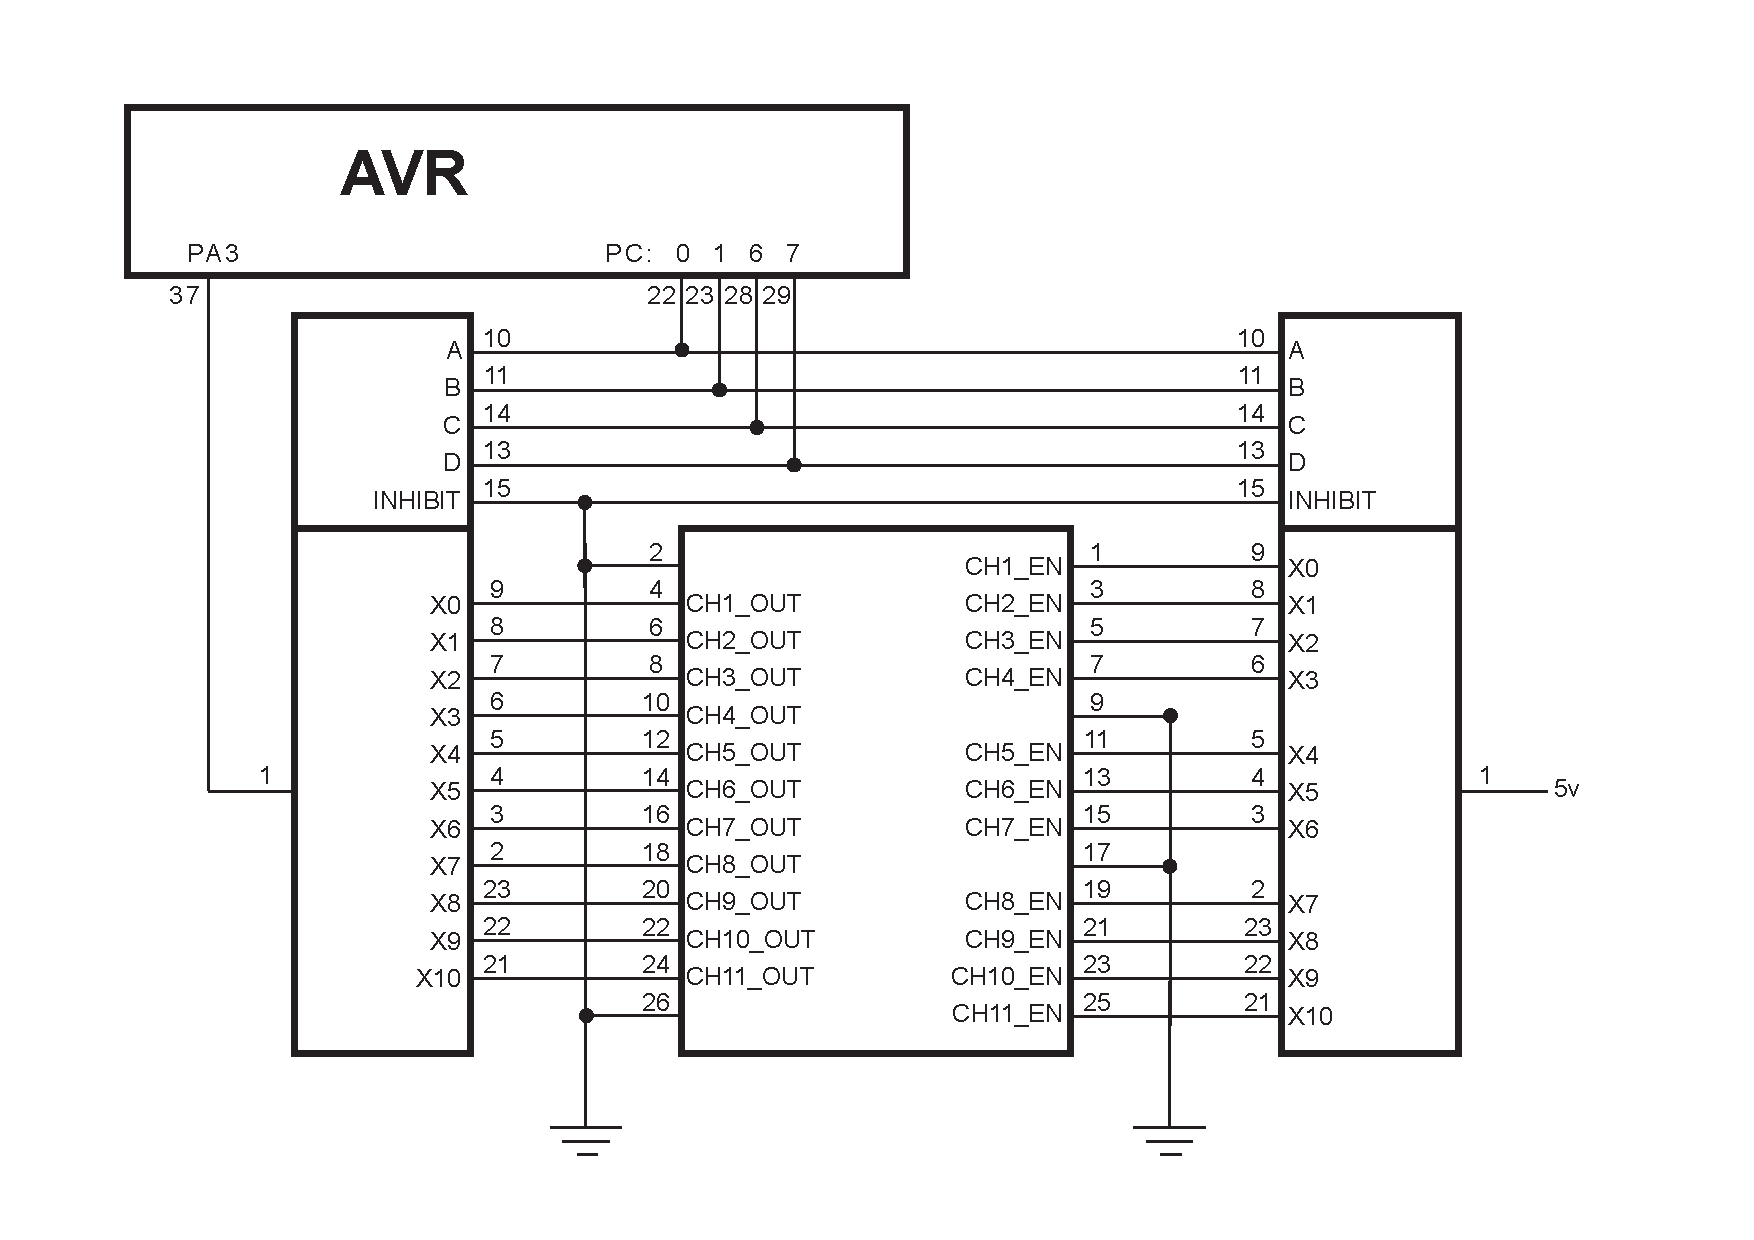
\includegraphics[angle=0,scale=0.5]{bilder/Uppkoppling_linjesensorer.pdf}
  \caption{Uppkoppling linjesensorer}
  \label{fig:Uppkoppling_linjesensorer}
\end{figure}

CH1 EN - CH11 EN är ingångar som leder signalen (logiskt ) vidare till lysdioderna. 
CH1  OUT - CH11 OUT Leder svarssignalen från transistorerna vidare mot styrenhetens 
AVR. Multiplexen och demultiplexen styrs med signalerna A - D från AVRen. Inhibit 
signalen är jordad då dataväljning alltid ska vara tillåten.



\subsubsection{Upptäckning av riktningsmarkeringar}
\label{sec:riktmark}
Då roboten är i en labyrint kommer linjeföljarsensorn huvudsakligen användas 
för att hitta riktningsmarkeringar. Dessa markeringar används för att visa i 
vilken riktning roboten ska färdas i nästkommande korsning.  I enlighet med 
banspecifikationen, se *REF BANSPEC*, är funktionen anpassad för att uppfatta 
följande signaler:

Högersväng visas med en tunn tejpmarkering följd av en tre gånger så tjock.
Vänstersväng visas genom en tjock tejpmarkering följd av en tre gånger så tunn.
Framåt visas genom två tunna tejpmarkeringar.

Vid varje uppdatering av samtliga linjeföljarsensorer görs en kontroll om de 
tre mittersta sensorerna ligger över tejp. Är så fallet så börjar antalet 
gånger linjesensorerna uppdateras att räknas. När de tre mittersta sensorerna 
inte längre ligger över tejp sparas antalet iterationer som sensorerna 
tillbringat över tejpen. Proceduren upprepas därefter och antalet iterationer 
jämförs för att se vilken tejpbit som var bredast, den första eller den andra
. Resultatet sparas därefter och efterfrågat kommando utförs i nästkommande 
korsning, se \ref{sec:upptackkorsning}.


\subsubsection{Avståndssensorer}
På roboten sitter fem avståndssensorer av typ GP2Y0A02YK som mäter avstånd
mellan 20 och 150 cm. Två sitter på robotens vänstra sida, två på högra och en
rakt fram. Dessa sensorer ger spänningsspikar varje millisekund så lågpassfilter
används för att få en jämnare signal utan spikar. Lågpassfiltren figur
har skärfrekvensen 54 Hz, se figur \ref{fig:lagpassfilter}. Utsignalen från
lågpassfiltrena är kopplade till port A på AVRen, se figur \ref{fig:PINsensor}.

\begin{figure}[H]
  \centering
 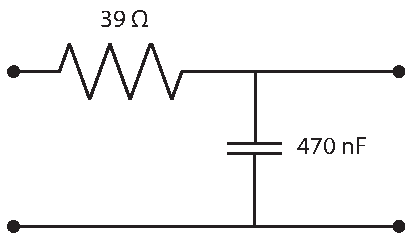
\includegraphics[angle=0,scale=0.5]{bilder/LPfilter.pdf}
  \caption{Lågpassfilter}
  \label{fig:lagpassfilter}
\end{figure}


\subsubsection{Upptäckning av korsningar och 90\degree svängar}
\label{sec:upptackkorsning}
Enligt specifikationen av den bana som roboten ska kunna följa, framgår det 
att det före alla korsningar ska finnas tejpmarkeringar som visar i vilken 
riktning roboten ska svänga, se \ref{sec:riktmark}. Roboten kommer att 
upptäcka korsningar om två av riktningarna höger, vänster och framåt visar 
mer än 80 cm.

Roboten kommer att upptäcka 90\degree svängar om det är längre än 80 cm åt 
höger eller vänster(inte båda), samt mindre än 35cm framåt.

Upptäcker roboten en korsning kommer det kommando som beskrivits av tidigare 
tejpmarkeringar att skickas till styrenheten. Datat som skickas är skrivet 
för att uppfattas som ett så kallat specialkommando, det vill säga 
styrenheten har en procedur som utförs utan att ta hänsyn till den reglerdata 
som skickas från sensorenheten. Märk att detta specialkommando innehåller en 
framkörning till mitten av korsningen, till skillnad från 90\degree svängar 
som utförs omedelbart.

Upptäcker korsningen en 90\degree sväng kommer ett annat specialkommando att 
utföras, där roboten svänger 90\degree åt det håll som avståndssensorerna 
visar har det längre avståndet.


\subsubsection{Display}
Robotens display-enhet är av typ \emph{LCD JM162A}. Displayen används för att visa avståndssensorernas värden. Eftersom sensorerna bara kan ge korrekta värden i intervallet 20-120 cm så kommer även displayen arbeta i detta intervall. Displayen arbetar i åtta databitarsläge och visar två rader med tecken. 

%Pinnar
Förutom de åtta databitarna som överförs för varje tecken till displayen så går ytterligare två signaler mellan sensorenhetens mikroprocessor och displayenheten: \emph{Enable} och \emph{Register select}. Enable-signalen signalerar till displayen att något ska skrivas ut, och Register select väljer mellan input-lägena 'data' och 'function'. Då det aldrig är någon data som läses från displayen så är pinnen \emph{R/W} konstant låg. 

%Kod
Sensorenheten har två funktioner som kan kallas för att skriva ut ett tecken på displayen. I funktionen \emph{char\_to\_display} anges parmetrarna vilket tecken (givet i ASCII-kod) som ska skrivas ut, samt vilken position på displayen som ska skrivas till. Denna funktion används för bokstäver. För att skriva ut sensorvärden används funktionen \emph{data\_to\_display}, vilken tar parametrarna för sensorvärdet i cm samt vilken sensor som skickat det. 

Sensorprocessorn har också en funktion för att konvertera cm-värdet till ASCII-kod, vilken används av \emph{data\_to\_display}.

\subsection{Mjukvara}

\subsubsection{AD}

\subsubsection{Linjesensor}


\subsubsection{Avståndsberäkning}


\subsubsection{Kommunikation}


\section{Styrenhet}

\subsection{Hårdvara}

\begin{figure}[H]
  \centering
 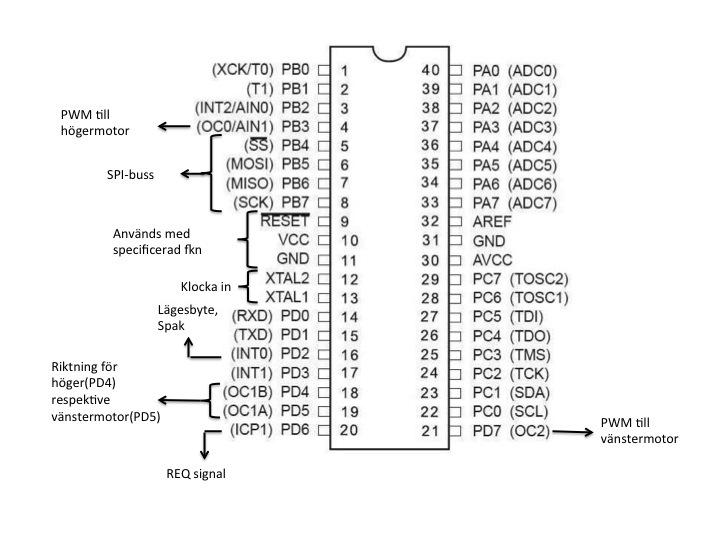
\includegraphics[angle=0,scale=0.5]{bilder/PIN_styr.jpg}
  \caption{Styrenhetens pin-anslutningar}
  \label{fig:PINstyr}
\end{figure}


\subsection{Mjukvara}

\subsubsection{Autonomt läge}

\subsection{Reglering}
Två olika regleralgoritmer används i roboten, en när roboten följer linjer och
en när roboten kör i labyrinter.
\subsubsection{Linjereglering}
TODO: Linjereglering
\subsubsection{Labyrintreglering}
Labyrintregleringen består av 3 olika delar med olika vikter,
en del som ser till att roboten går rakt (P-del), en del som ser till att
roboten håller sig i mitten av labyrinten (M-del) och en del som motverkar
svängningar (D-del).


P-delen använder sig av sidosensorerna för att hålla roboten parallell med
labyrintväggen. En vägg följs i taget, och kommer roboten för nära en vägg så
följs istället den andra väggen. Detta är den huvudsakliga regleringen och har
hög vikt.


M-delen använder sig av frontsensorerna för att hålla sig i mitten av
labyrinten, den försöker att hålla skillnaden mellan höger- och vänstersensorn
till 0. Om det bara finns en vägg att reglera på avaktiveras denna del. Då det
inte är helt avgörande om roboten är i mitten eller lite åt sidan i labyrinten
har denna del låg vikt.


D-delen ser till att roboten rör sig lugnt och inte börjar att oscillera i
labyrinten. Detta gör den genom att kika på skillnaden på sidosensorerna och är
den skillnaden stor så motverkar den P-delen. Eftersom D-delen reglerar på
relativt små skillnader har den hög vikt.

\label{reglering}

\section{PC mjukvara}
PC-mjukvaran har som uppgift att låta användaren kommunicera med roboten via ett
enkelt gränssnitt. Via PC-mjukvaran kan användaren få intressant information
från robotens olika moduler, t.ex avstånd till väggar eller vilket styrkommando
som nu utförs. PC-mjukvaran kommunicerar med roboten via blåtand.

\subsection{Implementering}

Mjukvaran är skriven i programspråket C och använder utöver Cs standardbibliotek
även gränssnittet BlueZ för att kommunicera via blåtand, biblioteket SDL för att
generera kommandon till roboten via tangentbordet samt NCurses för att
åskådliggöra information i terminalen på ett trevligt och överskådligt sätt..

Mjukvaran består av 2 huvuddelar, input\_control samt send\_receive. input\_control
hanterar knapptryckningar från användaren och genererar instruktioner att skicka
till roboten, intruktionen placeras sedan i en enkel databas (instr\_db).
send\_receive i sin tur läser in instruktionen från databasen och om användaren
har genererat en ny instruktion kommer denna skickas till roboten via blåtand
(instruktioner som redan skcikat till roboten kommer alltså inte att skickas
 igen), ifall instruktionen innehåller information om önskad hastighet på
roboten eller trimnivåer på motorerna så kommer detta också visas på skärmen.
När instruktionen skickats till roboten kommer send_receive invänta 2 databyte
från roboten (vilket kan vara sensorinfo, specialkommando el. dyl.) som sedan
kommer åskådligjöras på skärmen.
\subsection{Användande}

För att börja använda roboten startar man först programmet input_control, detta
initierar databasen instr\_db och ger användaren möjlighet att skapa
styrkommandon åt roboten med hjälp av tangentbordstryckningar. Sedan startar man
programmet send_receive som ansluter till roboten via blåtand och börjar skicka
samt ta emot data från roboten.

Då roboten befinner sig i fjärrstyrt läge används följande tangentbindningar för
att generera styrkommandon:
w - Kör framåt
s - Kör bakåt
a - rotera vänster
d - rotera höger
q - vänstersväng (mjuk kurva)
e - högersväng (mjuk kurva)
mellanslag - stanna roboten
pil upp - öka hastigheten, ingen effekt tills man skickar ett kommando som
utnyttjar hastigheten
pil ner - sänk hastigheten, ingen effekt tills man skickar ett kommando som
utnyttjar hastigheten.
pil höger - trim höger, öka effekten på höger motor en aning (små steg,
		användbart för finjustering)
pil vänster - trim vänster, öka effekten på vänster motor en aning (små steg,
		användbart för finjustering)
o - nollställ trim
esc - avsluta input\_control

För att avsluta send\_receive används (ctr + c) vilket kommer återställa
terminalen åt användaren.

% \subsection{Implementering}
% 
% Mjukvaran är skriven i programspråken C samt Tcl och använder utöver Cs standardbibliotek
% även gränssnittet BlueZ för att kommunicera via blåtand.
% 
% \subsection{Användande}
% 
% Mjukvaran kommer utgöras av ett fönster där användaren kan se information
% skickad från robotens sensorer och dess styrenhet samt skicka styrkommandon till
% roboten.
% 
% I fjärrstyrt läge kan användaren välja att använda de pilknappar som finns i
% fönstret för att styra roboten eller så kan användaren använda piltangenterna på
% tangentbordet.
% 
% I autonomt läge kommer gränssnittet visa information från robotens sensorer samt
% vilket styrkommando som roboten just nu utför.
% 
% Gränssnittet är enkelt att använda, kommandona är logiska och simpla och
% informationen från roboten visas på ett tydligt och lättförståeligt sätt.
% 

\section{Testning}
Integrationstestning görs för att kontrollera att alla gränssnitt fungerar som
de ska och att delsystemen svarar som förväntat på testdata. Vi kommer att
mestadels använda black-box testning men vid behov kommer vi att använda 
grey-box för att testa eventuella tillstånd som är svåra att nå.

Alla projektmedlemmar förväntas att göra sin egen enhetstestning alternativt se 
till att den blir gjord.

\subsection{Sensor- och kartenhet}
Sensorenheten är ganska simpel att testa då vi bara kan skicka in ett värde i
sensoränden och se om vi får ut ett bra värde när vi frågar efter det.

Kartenheten kan kontrolleras genom att skicka in en serie av sensorvärden och
se hur den omvandlar det till väggar på en karta.

\subsection{Styr- och kartenhet}
Styrenheten testas genom att alla olika styrkommandon skickas till den och vi
studerar dess utsignaler.

Bussen är enkelriktad så kartenheten kan inte skicka några meddelanden till
styrenheten.

\subsection{Robotsystemtest}
Vi systemtestar roboten genom att koppla ihop hela och se om den beter sig
specifikationsenligt när vi ger den kommandon, systemtestet är så beroende av
ett fungerande användargränssnitt i PC-mjukvaran att det inte kan genomföras
innan det är i alla fall så fullständigt att vi har ett kommandoradsgränssnitt.

\subsection{Systemintegrationstest}
Testning av hela systemet inklusive labyrint och PC-mjukvara. Vi kör runt
roboten i labyrinten och ser att kartan ritas korrekt på PC:n.

\section{Dokument}
Två dokument ska framställas och medfölja vid leveransen av roboten, en användarmanual samt teknisk dokumentation. All dokumentation skrivs enligt projektmodellen Lips.

\subsection{Användarmanual}
Användarmanualen ska fungera som en hjälp för den som använder den färdiga roboten. Den ska tydligt beskriva hur PC-gränssnittet fungerar och vilka kommandon som behövs för att styra roboten manuellt. Det ska även framgå hur man ställer om mellan autonomt och manuellt läge, samt under vilka förhållanden roboten kan förväntas kunna styra autonomt.

\subsection{Teknisk dokumentation}
Den tekniska dokumentationen ska till största del författas under tiden roboten konstrueras, och ska nogrannt beskriva varje delsystem. Dokumentationen är en del av slutleveransen, och det ska med hjälp av denna vara möjligt att bygga en kopia av roboten som konstrueras under projektet. Alla faser i konstruktionen som bidragit till den slutgiltiga roboten ska därmed dokumenteras och slutligen sammanställas till den tekniska dokumentationen.
%\section{Referenser}

%% --------------------------------------------------------------------------------------------------------------------------------------------
% APPENDIX - Blindtarm
%
% --matja307, 2012-05-06
%% --------------------------------------------------------------------------------------------------------------------------------------------

\section*{Appendix}
\appendix

\addcontentsline{toc}{section}{Appendix}

\lstset{inputencoding=utf8,
        language=c,
        linewidth=\textwidth,
        basicstyle=\scriptsize,
        numbers=left,
        stepnumber=1,
        tabsize=8,
        showtabs=false
}
\lstset{literate={å}{{\aa}}1
                {ä}{{\"a}}1
                {ö}{{\"o}}1
                {Å}{{\AA}}1
                {Ä}{{\"A}}1
                {Ö}{{\"O}}1
}


\section{Omvandlingsdiagram}
\label{appendix:cmomvandling}


\begin{figure}[H]
  \centering
 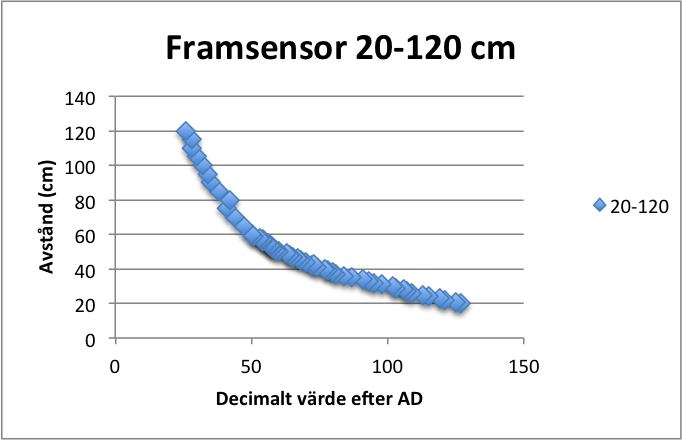
\includegraphics[angle=0,scale=1]{bilder/F_20_120.png}
  \caption{Framsensorn omvandling 20-120}
\end{figure}

\begin{figure}[H]
  \centering
 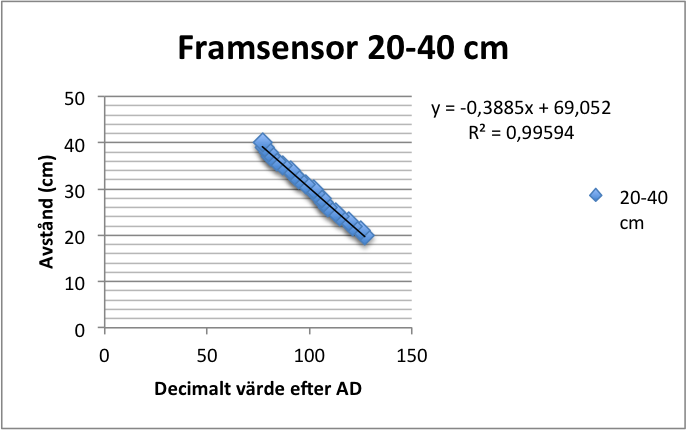
\includegraphics[angle=0,scale=1]{bilder/F_20_40.png}
  \caption{Framsensorn omvandling 20-40}
\end{figure}

\begin{figure}[H]
  \centering
 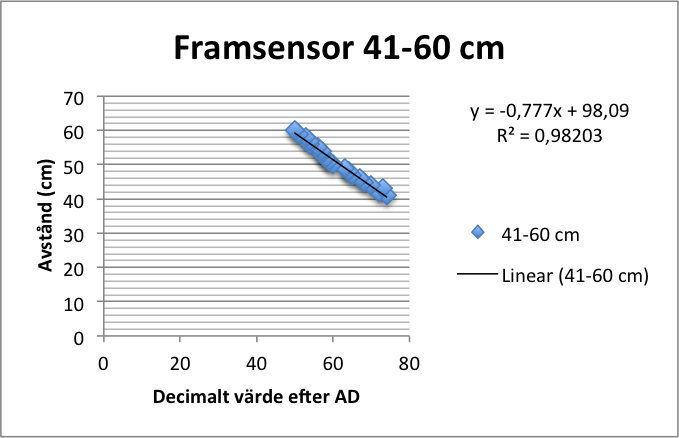
\includegraphics[angle=0,scale=1]{bilder/F_41_60.png}
  \caption{Framsensorns omvandling 41-60}
\end{figure}

\begin{figure}[H]
  \centering
 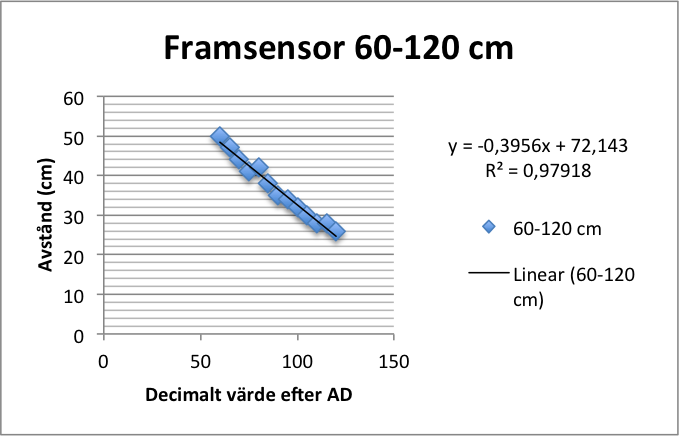
\includegraphics[angle=0,scale=1]{bilder/F_60_120.png}
  \caption{Framsensorn omvandling 60-120}
\end{figure}

\begin{figure}[H]
  \centering
 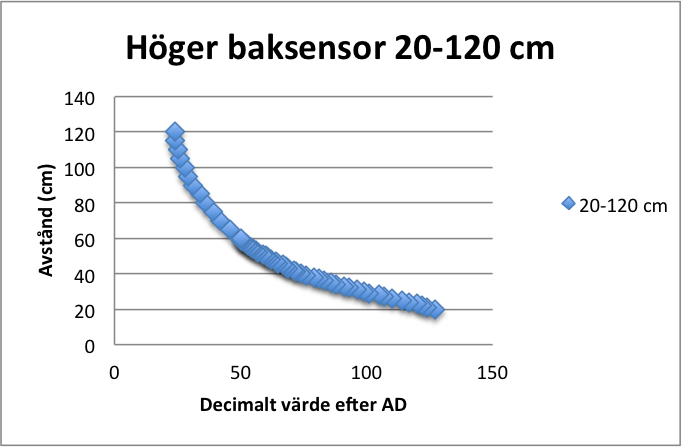
\includegraphics[angle=0,scale=1]{bilder/HB_20_120.png}
  \caption{Höger baksensor 20-120}
\end{figure}

\begin{figure}[H]
  \centering
 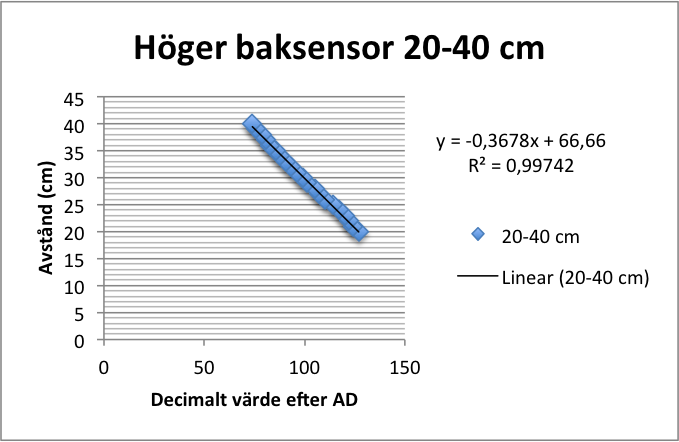
\includegraphics[angle=0,scale=1]{bilder/HB_20_40.png}
  \caption{Höger baksensor 20-40}
\end{figure}

\begin{figure}[H]
  \centering
 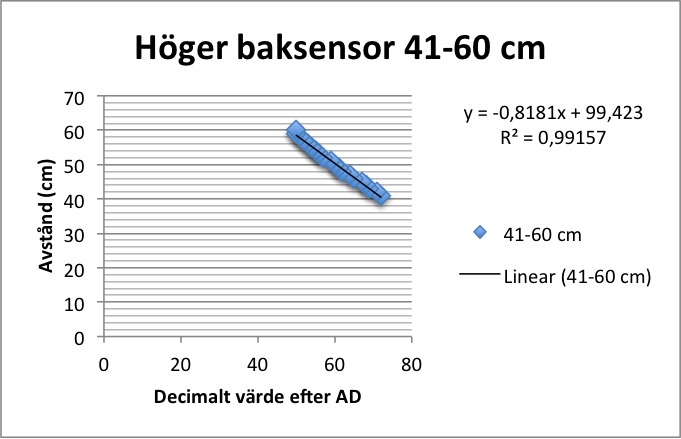
\includegraphics[angle=0,scale=1]{bilder/HB_41_60.png}
  \caption{Höger baksensor 41-60}
\end{figure}

\begin{figure}[H]
  \centering
 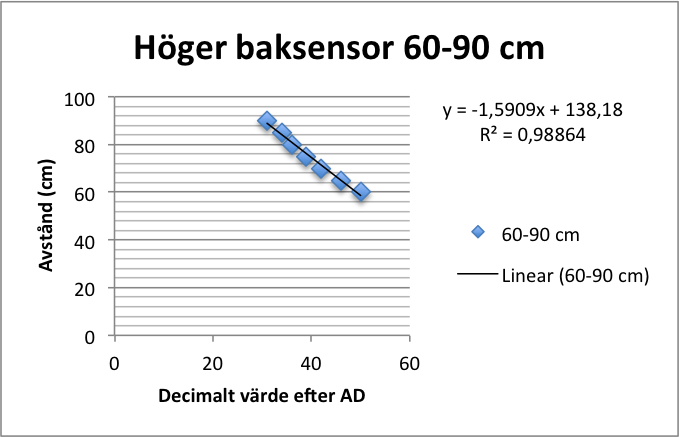
\includegraphics[angle=0,scale=1]{bilder/HB_60_90.png}
  \caption{Höger baksensor 60-90}
\end{figure}

\begin{figure}[H]
  \centering
 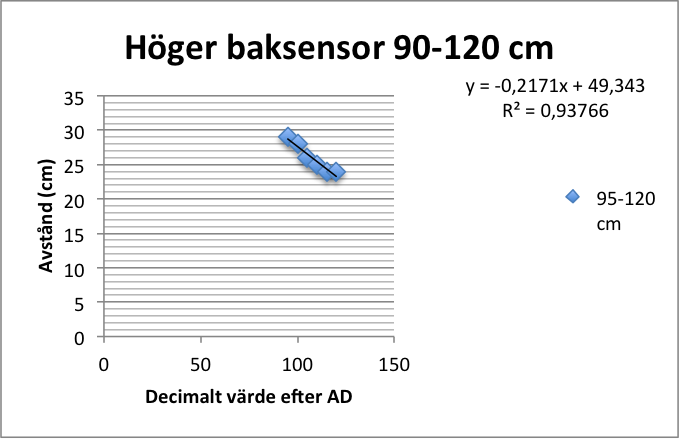
\includegraphics[angle=0,scale=1]{bilder/HB_90_120.png}
  \caption{Höger baksensor 90-120}
\end{figure}

\begin{figure}[H]
  \centering
 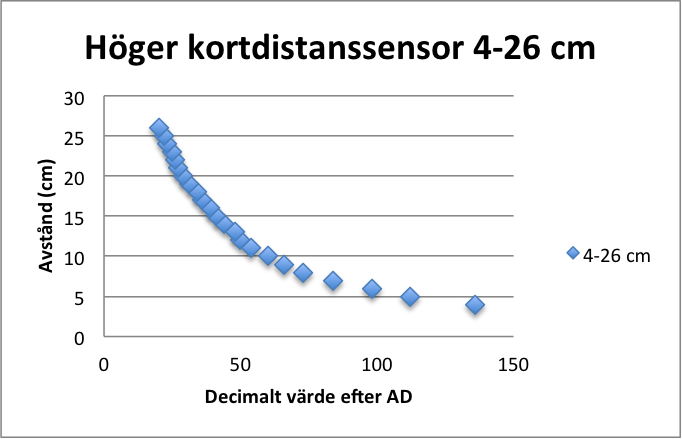
\includegraphics[angle=0,scale=1]{bilder/H_K_4_26.png}
  \caption{Höger kortdistanssensor 4-26}
\end{figure}

\begin{figure}[H]
  \centering
 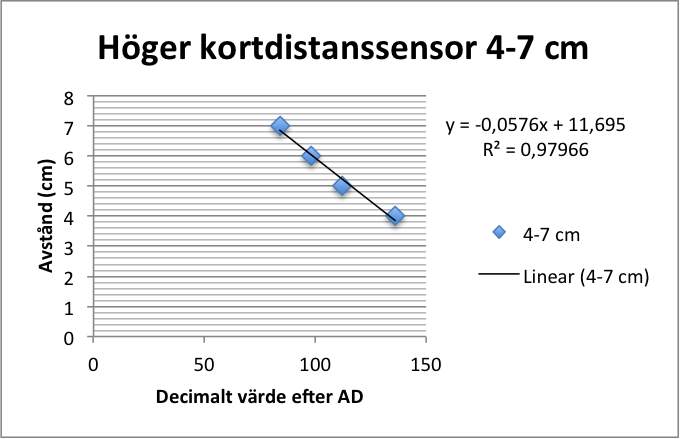
\includegraphics[angle=0,scale=1]{bilder/H_K_4_7png.png}
  \caption{Höger kortdistanssensor 4-7}
\end{figure}

\begin{figure}[H]
  \centering
 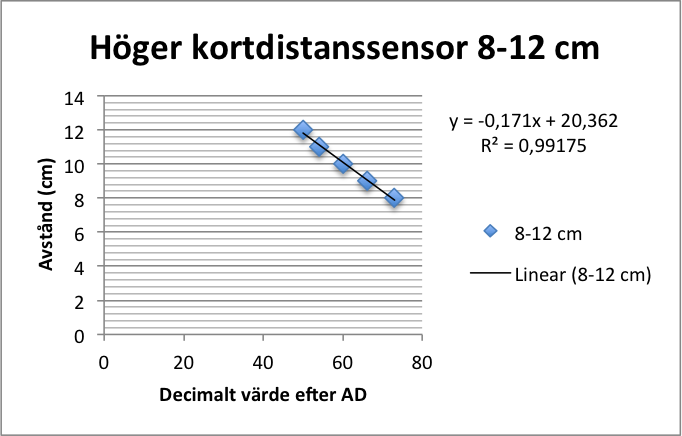
\includegraphics[angle=0,scale=1]{bilder/H_K_8_12.png}
  \caption{Höger kortdistanssensor 8-12}
\end{figure}

\begin{figure}[H]
  \centering
 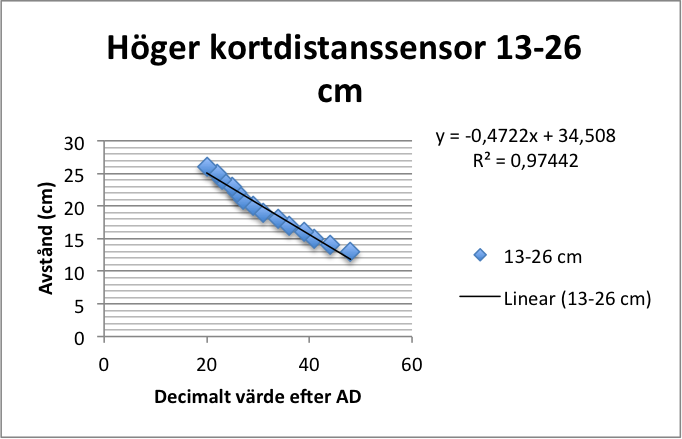
\includegraphics[angle=0,scale=1]{bilder/H_K_13_26.png}
  \caption{Höger kortdistanssensor 13-26}
\end{figure}

\begin{figure}[H]
  \centering
 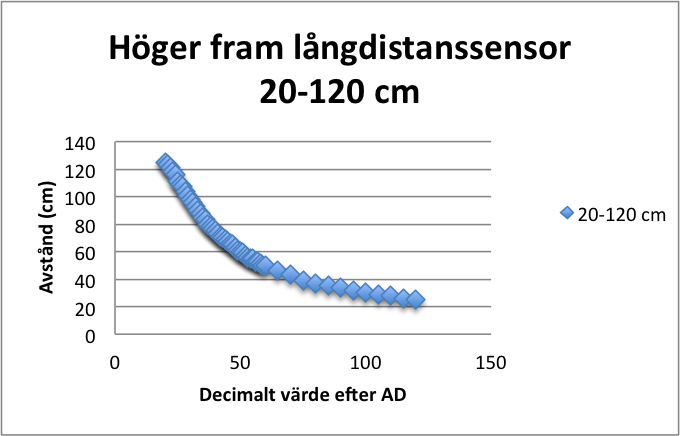
\includegraphics[angle=0,scale=1]{bilder/HF_20_120.png}
  \caption{Höger framsensor 20-120}
\end{figure}

\begin{figure}[H]
  \centering
 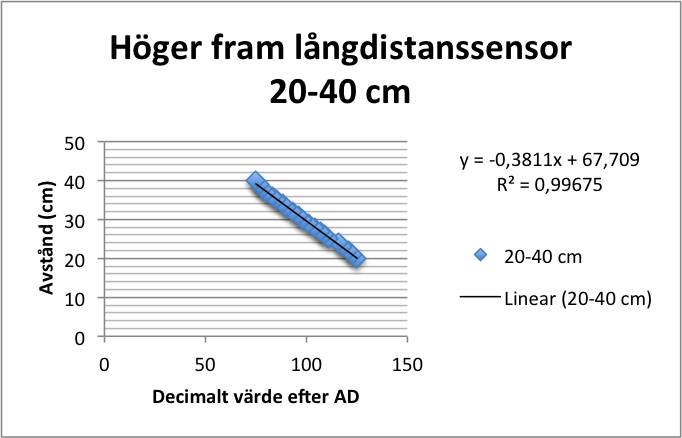
\includegraphics[angle=0,scale=1]{bilder/HF_20_40.png}
  \caption{Höger framsensor 20-40}
\end{figure}

\begin{figure}[H]
  \centering
 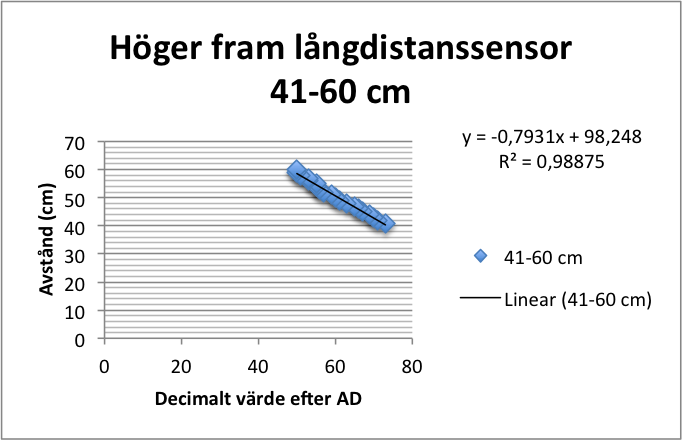
\includegraphics[angle=0,scale=1]{bilder/HF_41_60.png}
  \caption{Höger framsensor 41-60}
\end{figure}

\begin{figure}[H]
  \centering
 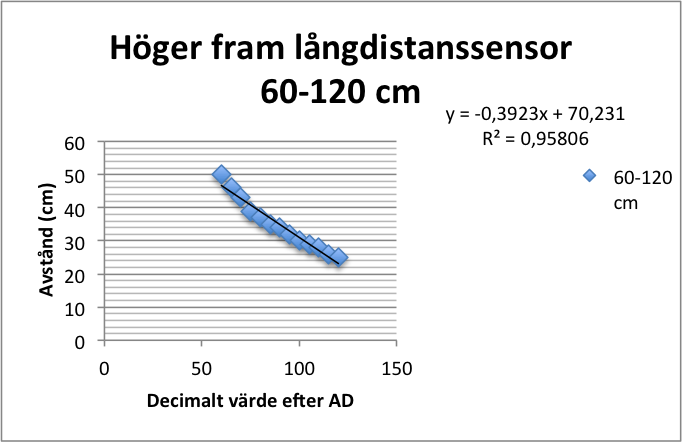
\includegraphics[angle=0,scale=1]{bilder/HF_60_120.png}
  \caption{Höger framsensor 60-120}
\end{figure}

\begin{figure}[H]
  \centering
 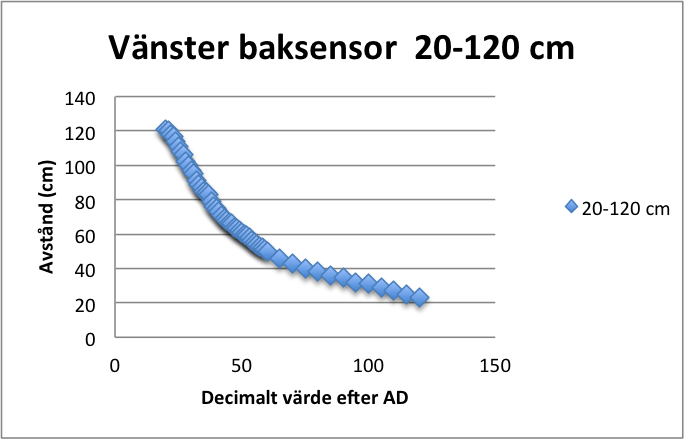
\includegraphics[angle=0,scale=1]{bilder/VB_20_120.png}
  \caption{Vänster baksensor 20-120}
\end{figure}

\begin{figure}[H]
  \centering
 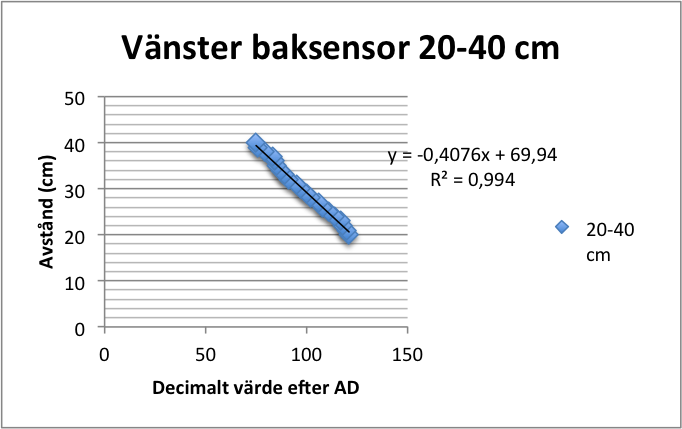
\includegraphics[angle=0,scale=1]{bilder/VB_20_40.png}
  \caption{Vänster baksensor 20-40}
\end{figure}


\begin{figure}[H]
  \centering
 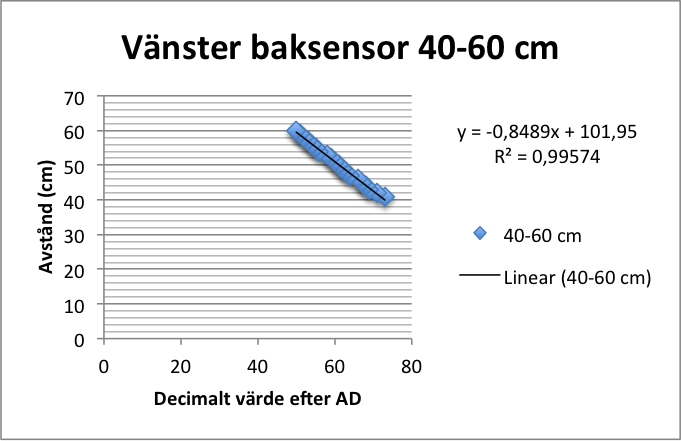
\includegraphics[angle=0,scale=1]{bilder/VB_40_60.png}
  \caption{Vänster baksensor 40-60}
\end{figure}

\begin{figure}[H]
  \centering
 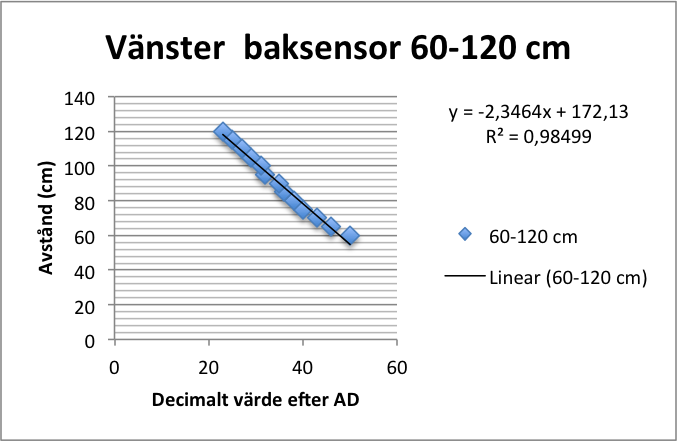
\includegraphics[angle=0,scale=1]{bilder/VB_60_120.png}
  \caption{Vänster baksensor 60-120}
\end{figure}

\begin{figure}[H]
  \centering
 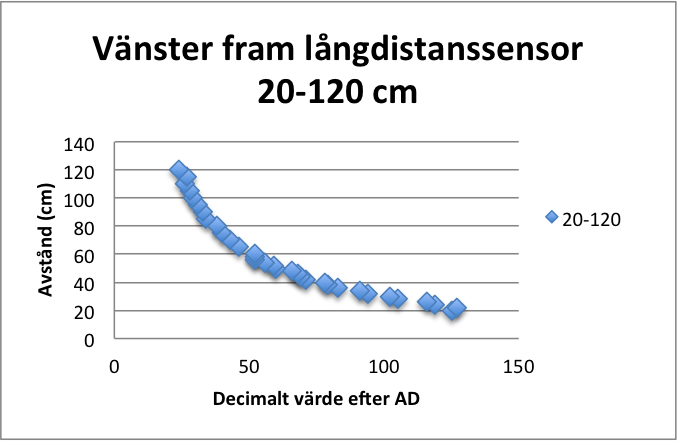
\includegraphics[angle=0,scale=1]{bilder/VF_20_120.png}
  \caption{Vänster framsensor 20-120}
\end{figure}

\begin{figure}[H]
  \centering
 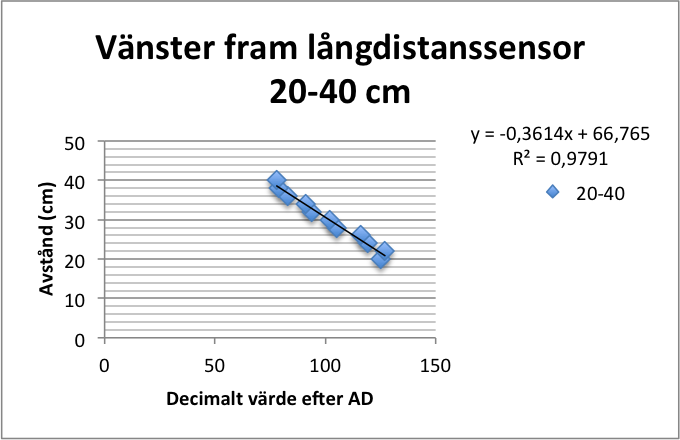
\includegraphics[angle=0,scale=1]{bilder/VF_20_40.png}
  \caption{Vänster framsensor 20-40}
\end{figure}

\begin{figure}[H]
  \centering
 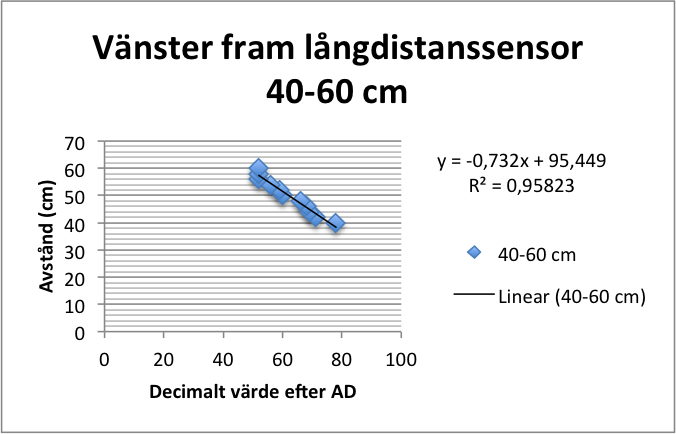
\includegraphics[angle=0,scale=1]{bilder/VF_40_60.png}
  \caption{Vänster framsensor 40-60}
\end{figure}

\begin{figure}[H]
  \centering
 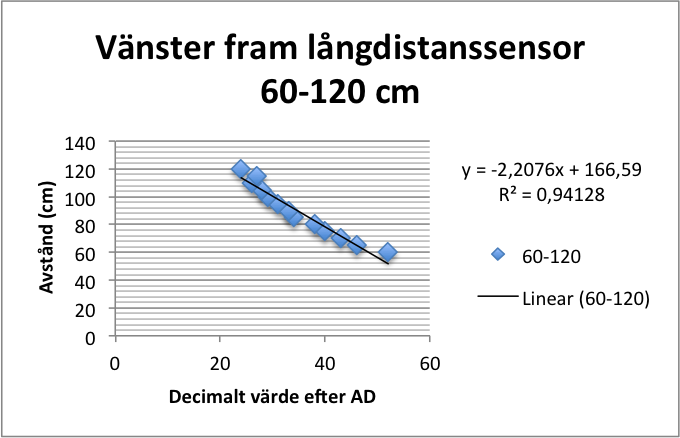
\includegraphics[angle=0,scale=1]{bilder/VF_60_120.png}
  \caption{Vänster framsensor 60-120}
\end{figure}






\subsection*{A \hspace*{1em} Kod}
\addcontentsline{toc}{subsection}{A \hspace*{1em} Kod}


%%%%%%%%%%%%%%%%%%%%%%%%%%%%%%%%%%%%%%%%%%%%%%%%%%%%%%%%%%%%%%%%%%%%%%%%%%%%%%%
% PC
% Kod till användargränssnittet
%%%%%%%%%%%%%%%%%%%%%%%%%%%%%%%%%%%%%%%%%%%%%%%%%%%%%%%%%%%%%%%%%%%%%%%%%%%%%%%
\subsubsection*{A.1 \hspace*{1em} PC}
\addcontentsline{toc}{subsubsection}{A.1 \hspace*{1em} PC}
\lstinputlisting[caption=input\_control,label=lst:input]{../../Kod/pc/input_control.c}
\lstinputlisting[caption=keypress.h,label=lst:keypress_h]{../../Kod/pc/keypress.h}
\lstinputlisting[caption=keypress.c,label=lst:keypress_c]{../../Kod/pc/keypress.c}
\lstinputlisting[caption=header.h,label=lst:header_h]{../../Kod/pc/header.h}
\lstinputlisting[caption=header.c,label=lst:header_c]{../../Kod/pc/header.c}
\lstinputlisting[caption=send\_receive.c,label=lst:sendrec_c]{../../Kod/pc/send_receive.c}
\lstinputlisting[caption=blue\_pc.h,label=lst:blue_h]{../../Kod/pc/blue_pc.h}
\lstinputlisting[caption=blue\_pc.c,label=lst:blue_c]{../../Kod/pc/blue_pc.c}
\lstinputlisting[caption=db.h,label=lst:db_h]{../../Kod/pc/db.h}
\lstinputlisting[caption=db.c,label=lst:db_c]{../../Kod/pc/db.c}
\lstinputlisting[caption=display.h,label=lst:display_h]{../../Kod/pc/display.h}
\lstinputlisting[caption=display.c,label=lst:display_c]{../../Kod/pc/display.c}

%%%%%%%%%%%%%%%%%%%%%%%%%%%%%%%%%%%%%%%%%%%%%%%%%%%%%%%%%%%%%%%%%%%%%%%%%%%%%%%
% Kommunikationsenhet
%%%%%%%%%%%%%%%%%%%%%%%%%%%%%%%%%%%%%%%%%%%%%%%%%%%%%%%%%%%%%%%%%%%%%%%%%%%%%%%
\subsubsection*{A.2 \hspace*{1em} Kommunikationsenhet}
\addcontentsline{toc}{subsubsection}{A.2 \hspace*{1em} Kommunikationsenhet}
\lstinputlisting[caption=komm\_main.c,label=lst:komm_main_c]{../../Kod/komm/komm_main.c}
\lstinputlisting[caption=komm\_init.c,label=lst:komm_init_c]{../../Kod/komm/komm_init.c}
\lstinputlisting[caption=bluetooth\_interrupt.c,%
label=lst:bluetooth_interrupt_c]{../../Kod/komm/bluetooth_interrupt.c}
\lstinputlisting[caption=komm\_SPI.c,label=lst:komm_SPI_c]{../../Kod/komm/komm_SPI.c}

%%%%%%%%%%%%%%%%%%%%%%%%%%%%%%%%%%%%%%%%%%%%%%%%%%%%%%%%%%%%%%%%%%%%%%%%%%%%%%%
% Styrenehet
%%%%%%%%%%%%%%%%%%%%%%%%%%%%%%%%%%%%%%%%%%%%%%%%%%%%%%%%%%%%%%%%%%%%%%%%%%%%%%%
\subsubsection*{A.3 \hspace*{1em} Styrenhet}
\addcontentsline{toc}{subsubsection}{A.3 \hspace*{1em} Styrenhet}
\lstinputlisting[caption=styr\_main.c,label=lst:styr_main_c]{../../Kod/styr/styr_main.c}
\lstinputlisting[caption=motor\_styrning.h,label=lst:motor_styrning_h]{../../Kod/styr/motor_styrning.h}
\lstinputlisting[caption=motor\_styrning.c,label=lst:motor_styrning_c]{../../Kod/styr/motor_styrning.c}
\lstinputlisting[caption=regulator.h,label=lst:regulator_h]{../../Kod/styr/regulator.h}
\lstinputlisting[caption=regulator.c,label=lst:regulator_c]{../../Kod/styr/regulator.c}
\lstinputlisting[caption=styr\_specialkommando.h,label=lst:styr_specialkommando_h]{../../Kod/styr/styr_specialkommando.h}
\lstinputlisting[caption=styr\_specialkommando.c,label=lst:styr_specialkommando_c]{../../Kod/styr/styr_specialkommando.c}
\lstinputlisting[caption=styr\_tolka\_data.h,label=lst:styr_tolka_data_h]{../../Kod/styr/styr_tolka_data.h}
\lstinputlisting[caption=styr\_tolka\_data.c,label=lst:styr_tolka_data_c]{../../Kod/styr/styr_tolka_data.c}
\lstinputlisting[caption=styr\_SPI.h,label=lst:styr_SPI_h]{../../Kod/styr/styr_SPI.h}
\lstinputlisting[caption=styr\_SPI.c,label=lst:styr_SPI_c]{../../Kod/styr/styr_SPI.c}

%%%%%%%%%%%%%%%%%%%%%%%%%%%%%%%%%%%%%%%%%%%%%%%%%%%%%%%%%%%%%%%%%%%%%%%%%%%%%%%
% Sensorenhet
%%%%%%%%%%%%%%%%%%%%%%%%%%%%%%%%%%%%%%%%%%%%%%%%%%%%%%%%%%%%%%%%%%%%%%%%%%%%%%%
\subsubsection*{A.4 \hspace*{1em} Sensorenhet}
\addcontentsline{toc}{subsubsection}{A.4 \hspace*{1em} Sensorenhet}
\lstinputlisting[caption=sensor.c,label=lst:sensor_c]{../../Kod/sensor/sensor.c}
\lstinputlisting[caption=sensor\_init.h,label=lst:sensor_init_h]{../../Kod/sensor/sensor_init.h}
\lstinputlisting[caption=sensor\_init.c,label=lst:sensor_init_c]{../../Kod/sensor/sensor_init.c}
\lstinputlisting[caption=sensor\_ad.h,label=lst:sensor_ad_h]{../../Kod/sensor/sensor_ad.h}
\lstinputlisting[caption=sensor\_ad.c,label=lst:sensor_ad_c]{../../Kod/sensor/sensor_ad.c}
\lstinputlisting[caption=sensorvarde\_omvandling.h,label=lst:sensorvarde_omvandling_h]{../../Kod/sensor/sensorvarde_omvandling.h}
\lstinputlisting[caption=sensorvarde\_omvandling.c,label=lst:sensorvarde_omvandling_c]{../../Kod/sensor/sensorvarde_omvandling.c}
\lstinputlisting[caption=displayenhet.h,label=lst:displayenhet_h]{../../Kod/sensor/displayenhet.h}
\lstinputlisting[caption=displayenhet.c,label=lst:displayenhet_c]{../../Kod/sensor/displayenhet.c}
\lstinputlisting[caption=linjeskillnad.h,label=lst:linjeskillnad_h]{../../Kod/sensor/linjeskillnad.h}
\lstinputlisting[caption=linjeskillnad.c,label=lst:linjeskillnad_c]{../../Kod/sensor/linjeskillnad.c}
\lstinputlisting[caption=upptack\_tejp.h,label=lst:upptack_tejp_h]{../../Kod/sensor/upptack_tejp.h}
\lstinputlisting[caption=upptack\_tejp.c,label=lst:upptack_tejp_c]{../../Kod/sensor/upptack_tejp.c}
\lstinputlisting[caption=special.h,label=lst:special_h]{../../Kod/sensor/special.h}
\lstinputlisting[caption=special.c,label=lst:special_c]{../../Kod/sensor/special.c}
\lstinputlisting[caption=sensor\_spi.h,label=lst:sensor_spi_h]{../../Kod/sensor/sensor_spi.h}
\lstinputlisting[caption=sensor\_spi.c,label=lst:sensor_spi_c]{../../Kod/sensor/sensor_spi.c}

\subsection*{B \hspace*{1em} Kopplingsschema}
\addcontentsline{toc}{subsection}{B \hspace*{1em} Kopplingsschema}
\begin{figure}[H]
 \centering
 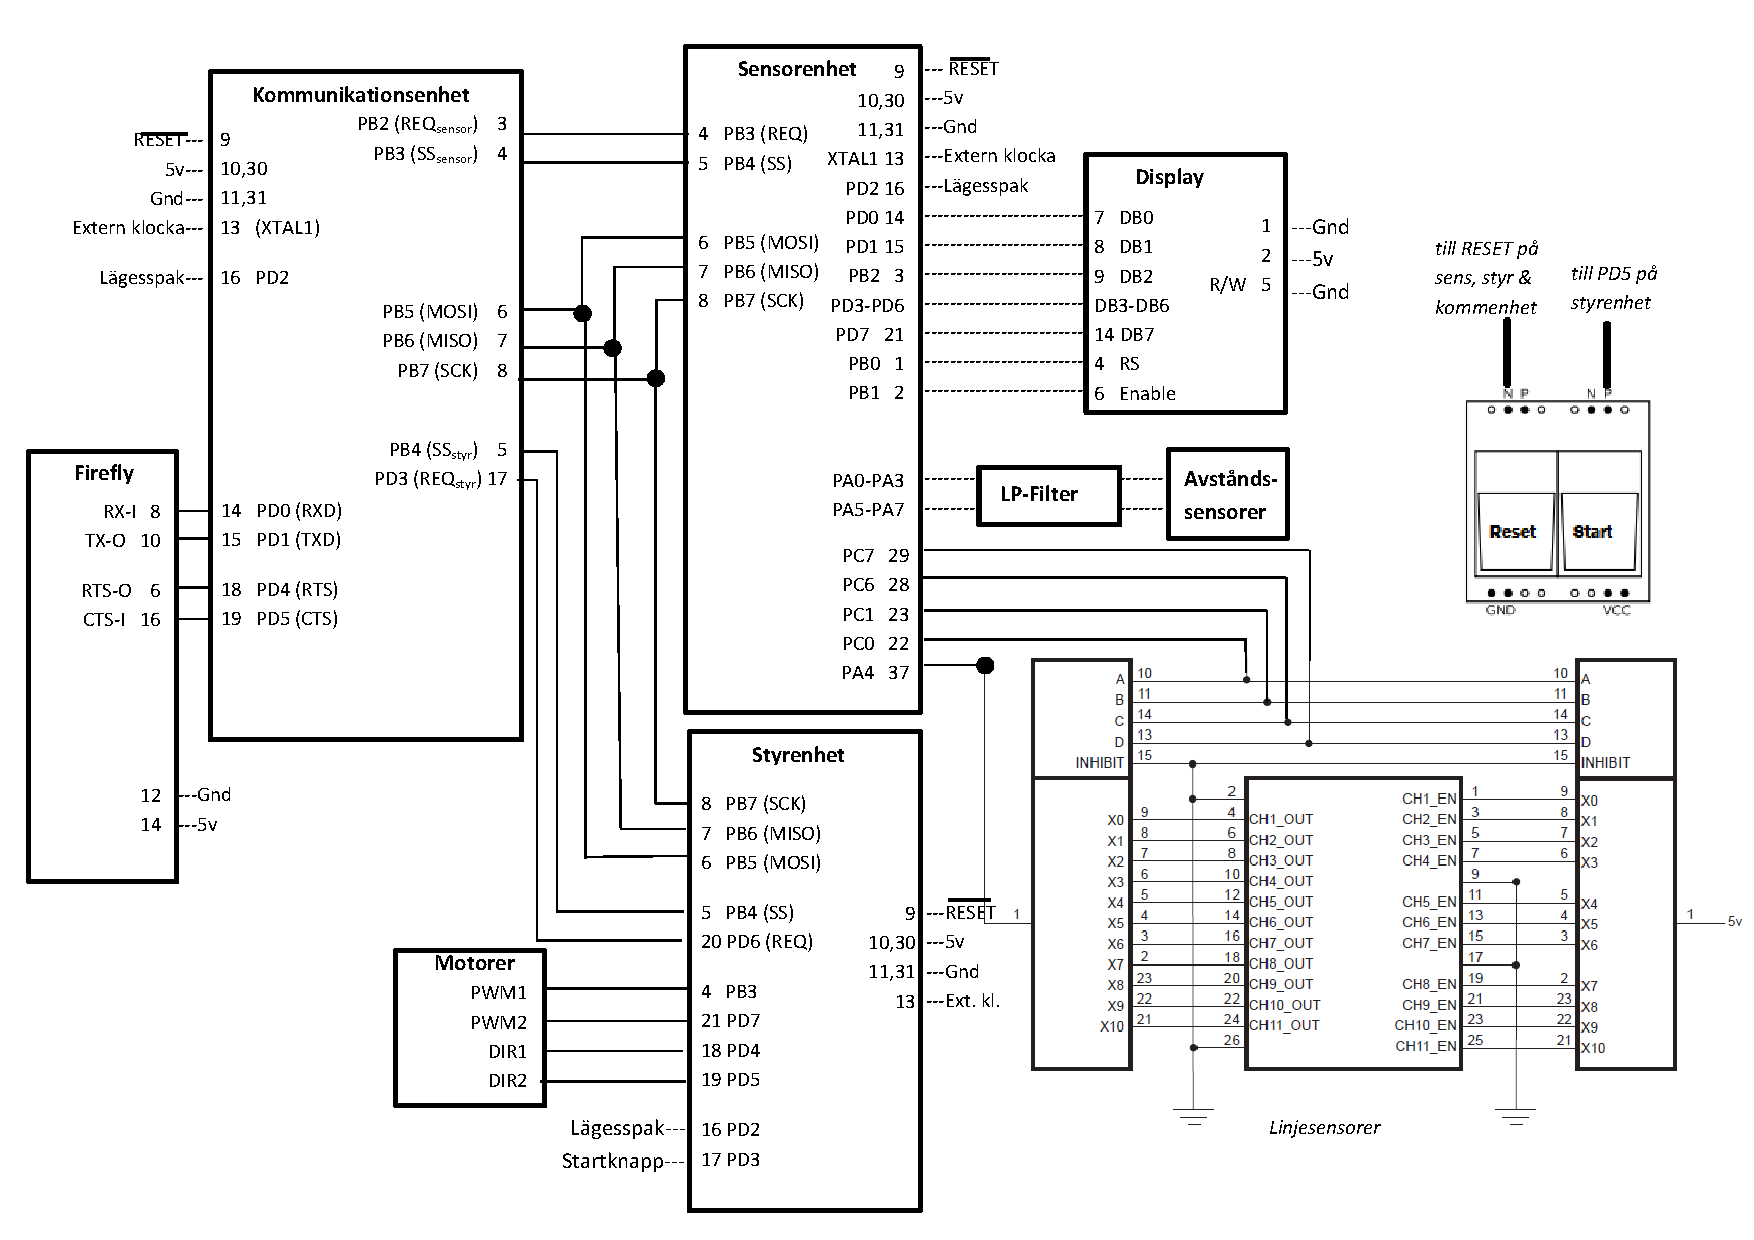
\includegraphics[angle=270,scale=0.75]{bilder/kopplingsschema.pdf}
  \caption{Kopplingsschema för systemet}
  %\label{fig:system}
\end{figure}


\end{document} 
%%% Local Variables: 
%%% mode: latex
%%% TeX-master: t
%%% End: 
